\documentclass{standalone}
\usepackage{tikz}
\begin{document}
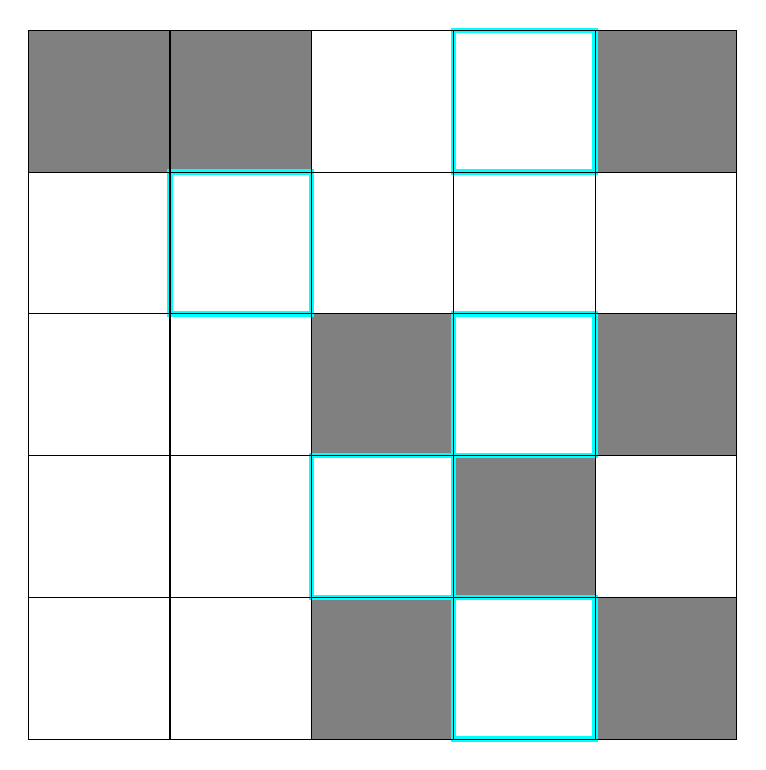
\begin{tikzpicture}[x=1.8cm, y=1.8cm]
    % Define colors
    \definecolor{grayfilled}{rgb}{0.5, 0.5, 0.5}
    \definecolor{cyanborder}{rgb}{0, 1, 1}
    % Fill gray squares
    \foreach \i/\j in {0/4, 1/4, 2/2, 2/0, 3/1, 4/0, 4/2, 4/4} {
        \fill[grayfilled] (\i,\j) rectangle ++(1,1);
    }
    % Cyan border squares
    \foreach \i/\j in {1/3, 2/1, 3/0, 3/2, 3/4} {
        \draw[line width=2pt, cyanborder] (\i,\j) rectangle ++(1,1);
    }
    % Draw grid
    \foreach \i in {0,1,...,5} {
        \draw (\i,0) -- (\i,5);
        \draw (0,\i) -- (5,\i);
    }
\end{tikzpicture}
\end{document}